%!TeX root=../wowtop.tex

\ArtChapter[The Stillness]{22head}

\lettrine[lines=4]{M}{y} first act before I went into the pantry was to fasten the door between the kitchen and the scullery. But the pantry was empty; every scrap of food had gone. Apparently, the Martian had taken it all on the previous day. At that discovery I despaired for the first time. I took no food, or no drink either, on the eleventh or the twelfth day.

At first my mouth and throat were parched, and my strength ebbed sensibly. I sat about in the darkness of the scullery, in a state of despondent wretchedness. My mind ran on eating. I thought I had become deaf, for the noises of movement I had been accustomed to hear from the pit had ceased absolutely. I did not feel strong enough to crawl noiselessly to the peephole, or I would have gone there.

On the twelfth day my throat was so painful that, taking the chance of alarming the Martians, I attacked the creaking rain-water pump that stood by the sink, and got a couple of glassfuls of blackened and tainted rain water. I was greatly refreshed by this, and emboldened by the fact that no enquiring tentacle followed the noise of my pumping.

During these days, in a rambling, inconclusive way, I thought much of the curate and of the manner of his death.

On the thirteenth day I drank some more water, and dozed and thought disjointedly of eating and of vague impossible plans of escape. Whenever I dozed I dreamt of horrible phantasms, of the death of the curate, or of sumptuous dinners; but, asleep or awake, I felt a keen pain that urged me to drink again and again. The light that came into the scullery was no longer grey, but red. To my disordered imagination it seemed the colour of blood.

On the fourteenth day I went into the kitchen, and I was surprised to find that the fronds of the red weed had grown right across the hole in the wall, turning the half-light of the place into a crimson-coloured obscurity.

It was early on the fifteenth day that I heard a curious, familiar sequence of sounds in the kitchen, and, listening, identified it as the snuffing and scratching of a dog. Going into the kitchen, I saw a dog's nose peering in through a break among the ruddy fronds. This greatly surprised me. At the scent of me he barked shortly.

I thought if I could induce him to come into the place quietly I should be able, perhaps, to kill and eat him; and in any case, it would be advisable to kill him, lest his actions attracted the attention of the Martians.

I crept forward, saying »Good dog!« very softly; but he suddenly withdrew his head and disappeared.

I listened—I was not deaf—but certainly the pit was still. I heard a sound like the flutter of a bird's wings, and a hoarse croaking, but that was all.

For a long while I lay close to the peephole, but not daring to move aside the red plants that obscured it. Once or twice I heard a faint pitter-patter like the feet of the dog going hither and thither on the sand far below me, and there were more birdlike sounds, but that was all. At length, encouraged by the silence, I looked out.

Except in the corner, where a multitude of crows hopped and fought over the skeletons of the dead the Martians had consumed, there was not a living thing in the pit.

\begin{figure}[tbp]
\centering
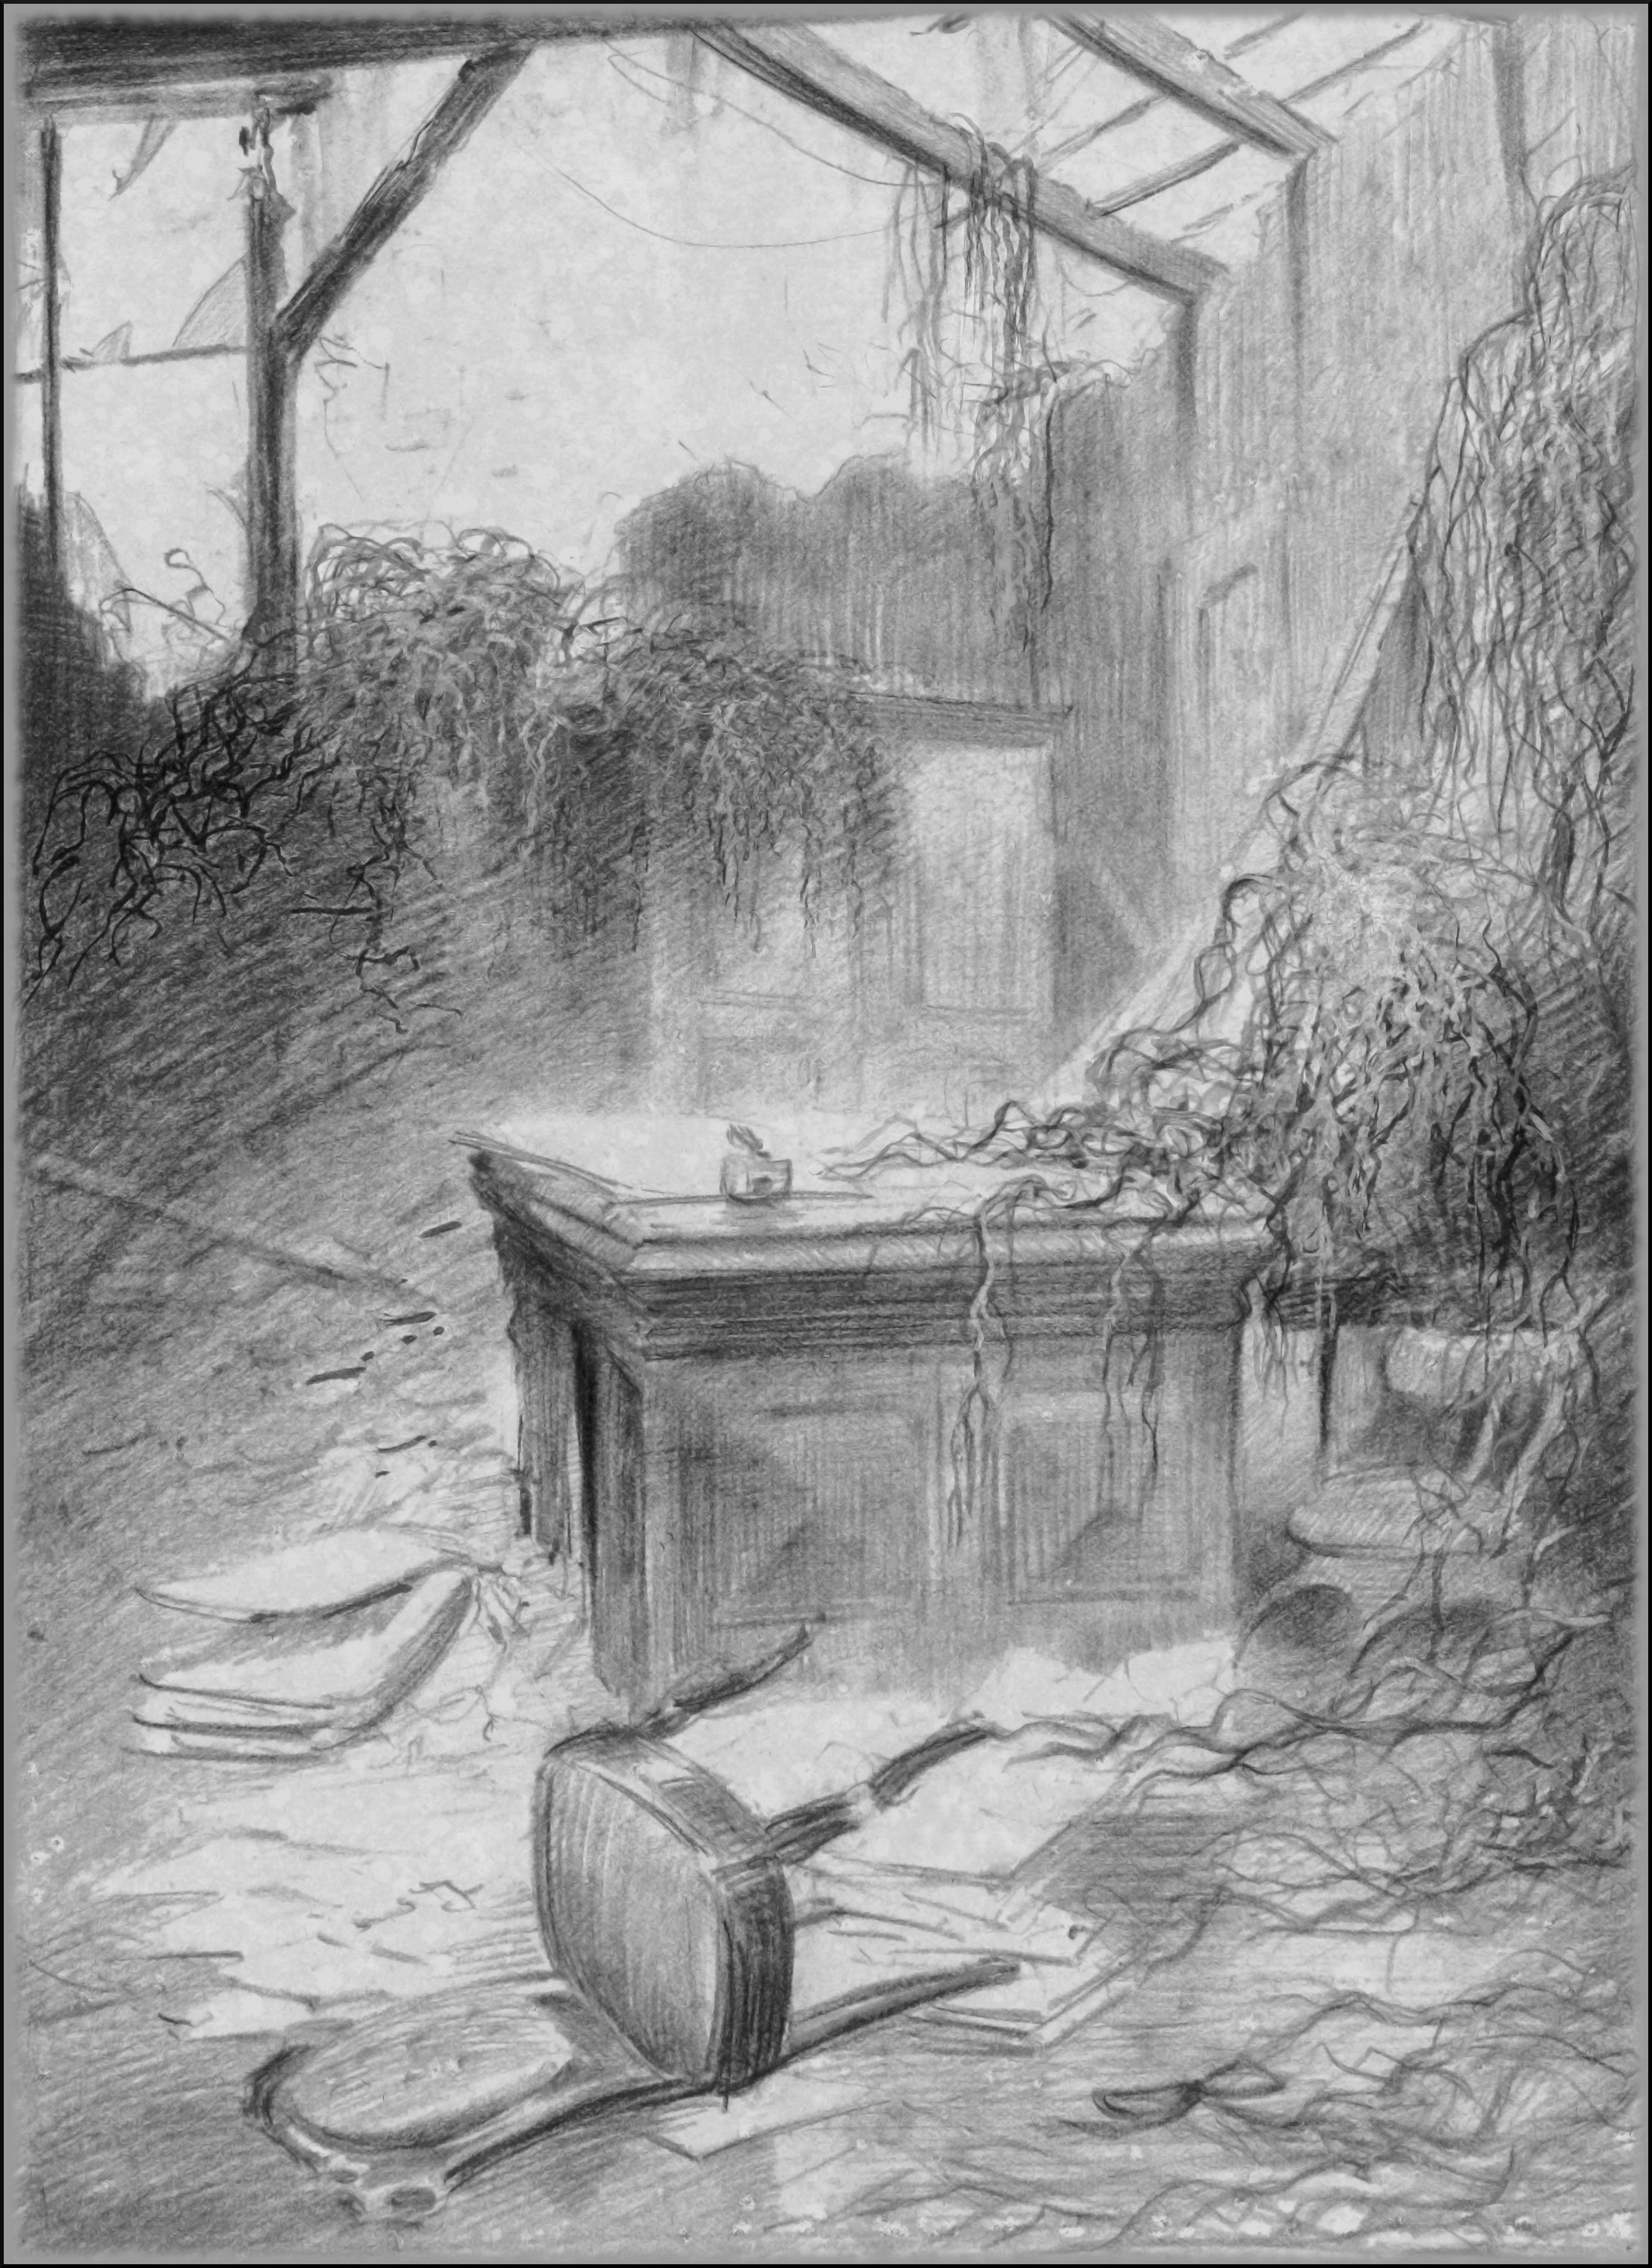
\includegraphics[width=\linewidth]{22roofless}
\caption{The neighbouring houses had all been wrecked}
\end{figure}

I stared about me, scarcely believing my eyes. All the machinery had gone. Save for the big mound of greyish-blue powder in one corner, certain bars of aluminium in another, the black birds, and the skeletons of the killed, the place was merely an empty circular pit in the sand.

Slowly I thrust myself out through the red weed, and stood upon the mound of rubble. I could see in any direction save behind me, to the north, and neither Martians nor sign of Martians were to be seen. The pit dropped sheerly from my feet, but a little way along the rubbish afforded a practicable slope to the summit of the ruins. My chance of escape had come. I began to tremble.

I hesitated for some time, and then, in a gust of desperate resolution, and with a heart that throbbed violently, I scrambled to the top of the mound in which I had been buried so long.

I looked about again. To the northward, too, no Martian was visible.

When I had last seen this part of Sheen in the daylight it had been a straggling street of comfortable white and red houses, interspersed with abundant shady trees. Now I stood on a mound of smashed brickwork, clay, and gravel, over which spread a multitude of red cactus-shaped plants, knee-high, without a solitary terrestrial growth to dispute their footing. The trees near me were dead and brown, but further a network of red thread scaled the still living stems.

The neighbouring houses had all been wrecked, but none had been burned; their walls stood, sometimes to the second story, with smashed windows and shattered doors. The red weed grew tumultuously in their roofless rooms. Below me was the great pit, with the crows struggling for its refuse. A number of other birds hopped about among the ruins. Far away I saw a gaunt cat slink crouchingly along a wall, but traces of men there were none.



The day seemed, by contrast with my recent confinement, dazzlingly bright, the sky a glowing blue. A gentle breeze kept the red weed that covered every scrap of unoccupied ground gently swaying. And oh! the sweetness of the air!

\begin{figure}[bh!]
\centering

\includegraphics[width=.4\textwidth]{22tailpiece}
%\captionlistentry{Tailpiece to Chapter \thechapter}
\end{figure}
\enlargethispage{2\baselineskip}